%%%%%%%%%%%%%%%%%%%%%%%%%%%%%%%%%%%%%%%%%%%%%%%%%%%%%%%%%%%%%%%%%%%%%%%%
% Plantilla TFG/TFM
% Escuela Politécnica Superior de la Universidad de Alicante
% Realizado por: Jose Manuel Requena Plens
% Contacto: info@jmrplens.com / Telegram:@jmrplens
%%%%%%%%%%%%%%%%%%%%%%%%%%%%%%%%%%%%%%%%%%%%%%%%%%%%%%%%%%%%%%%%%%%%%%%%

\chapter{Experimentación}
\label{experimentacion}

A partir de este momento, se va a mostrar toda la experimentación realizada en este proyecto con la red, para ello se va a comenzar comentando los arreglos que se hicieron necesarios para poder realizar la comparación de los modelos.

\section{Preprocesado de los modelos de Tech4diet[\cite{tech}]}

Los modelos generados por Tech4diet[\cite{tech}], tienen suciedad en la parte de los pies, pues representan la plataforma que pisas para hacerte la reconstrucción del cuerpo.

Este proceso fue necesario para tratar de tener una mejor comparativa de modelos obtenidos por PIFu[\cite{pifu}], dado que hasta la alineación era compleja por este motivo. El proceso se realizó con la herramienta de Blender[\cite{blender}], se eliminaron las partes sobrantes como se puede ver en la siguiente imagen.

\begin{figure}[H]
	\centering
	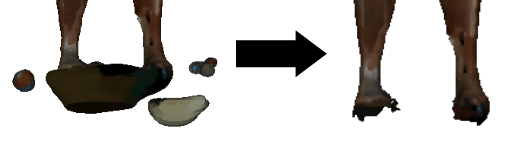
\includegraphics[scale=0.8]{imagenes/experimentacion1.png}
	\caption{Preprocesado en modelo Tech4diet[\cite{tech}]}
	\label{fig:figura9}
\end{figure}

Como se puede ver en la figura \ref{fig:figura9} se ha limpiado la plataforma, que no forma parte del cuerpo humano.

\section{Escalado de los modelos obtenidos con el método de PIFu[\cite{pifu}]}

Para poder analizar los modelos se ha de tener en cuenta las medidas, y en este caso los modelos obtenidos por PIFu[\cite{pifu}] todos tienen el mismo tamaño como se puede ver en la figura \ref{fig:figura12}. 
\begin{figure}[H]
	\centering
	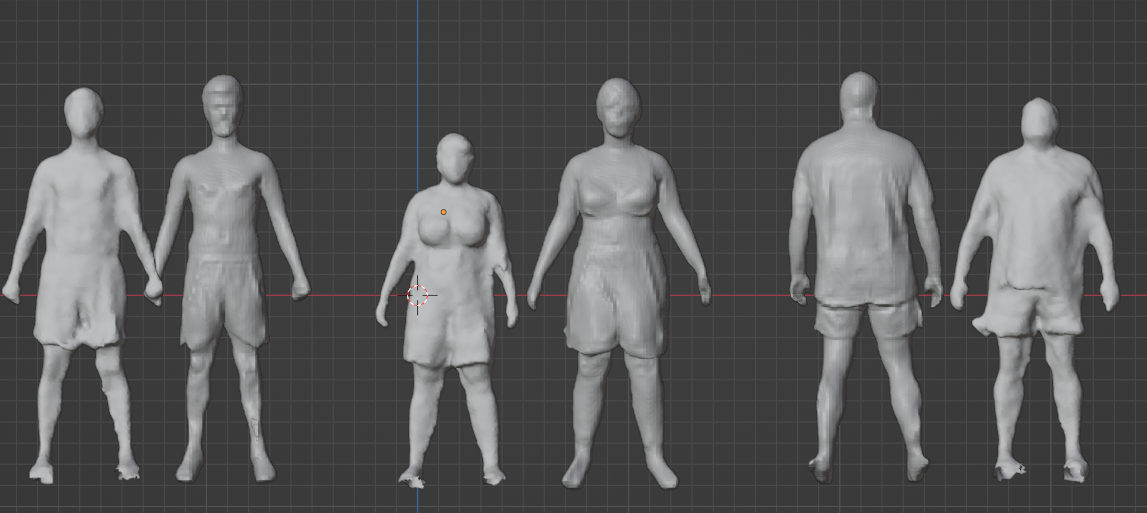
\includegraphics[scale=0.4]{imagenes/difaltura.png}
	\caption{Diferencia de altura de los modelos, el modelo de la derecha de cada pareja es el generado por la red[\cite{pifu}]}
	\label{fig:figura12}
\end{figure}

En el cálculo de distancias de Chamfer se necesita que estos modelos ya tengan la misma altura para así poder obtener un resultado más realista.
\begin{figure}[H]
	\centering
	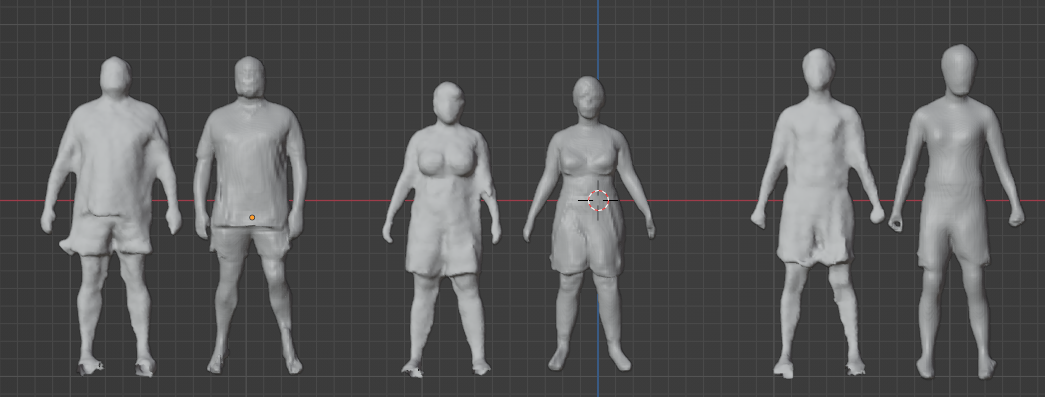
\includegraphics[scale=0.4]{imagenes/difaltura1.png}
	\caption{Diferencia de altura de los modelos, ya escalados }
	\label{fig:figura13}
\end{figure}

La figura \ref{fig:figura13} muestra el cambio obtenido después del escalado realizado con la aplicación Blender[\cite{blender}]

\section{Creación de las nubes de punto correspondientes a cada modelo}

En el cálculo de la distancia de Chamfer es necesario tener las nubes de punto de los modelos 3D, porque cómo se puede ver en el código \ref{cod:3} se calcula con $arrays$, y las nubes de punto son realmente $arrays$ con las coordenadas $x$, $y$ y $z$ de cada punto (también tienen la información del color y las normales por coordenada, pero hemos eliminado toda esta información, ya que el análisis es de la forma del cuerpo). Para ello se utilizo la aplicación MeshLab[\cite{MeshLab}] y se exportó cada uno de los modelos en formato ply.

\section{Alineamiento de modelos}

Para poder calcular la distancia de Hausdorff se necesita que los modelos estén alineados, dado que se va a calcular en MeshLab[\cite{MeshLab}], este proceso también se va a realizar en este software.

Este proceso se hace mediante la herramienta $Align$, y con esta herramienta aparece una ventana donde nos aparecen diferentes opciones, lo primero que haremos será seleccionar el modelo obtenido por Tech4diet[\cite{tech}], dado que es el modelo que se usa para comprobar los resultados obtenidos y se elige la opción $Glue Mesh Here$, esto lo que hace es que la malla se va a quedar fija en el lugar y la otra malla es la que se va a alinear con esta. Para poder alinearla se selecciona la opción $Point Based Glueling$.

Una vez elegida la opción para alinear, aparece otra ventana donde salen los dos modelos como se puede ver en la figura \ref{fig:figura10}, aquí se eligen punto a punto en ambas mallas y a la vez seleccionamos la opción de escalado para que ambos modelos tengan el mismo tamaño.

\begin{figure}[H]
	\centering
	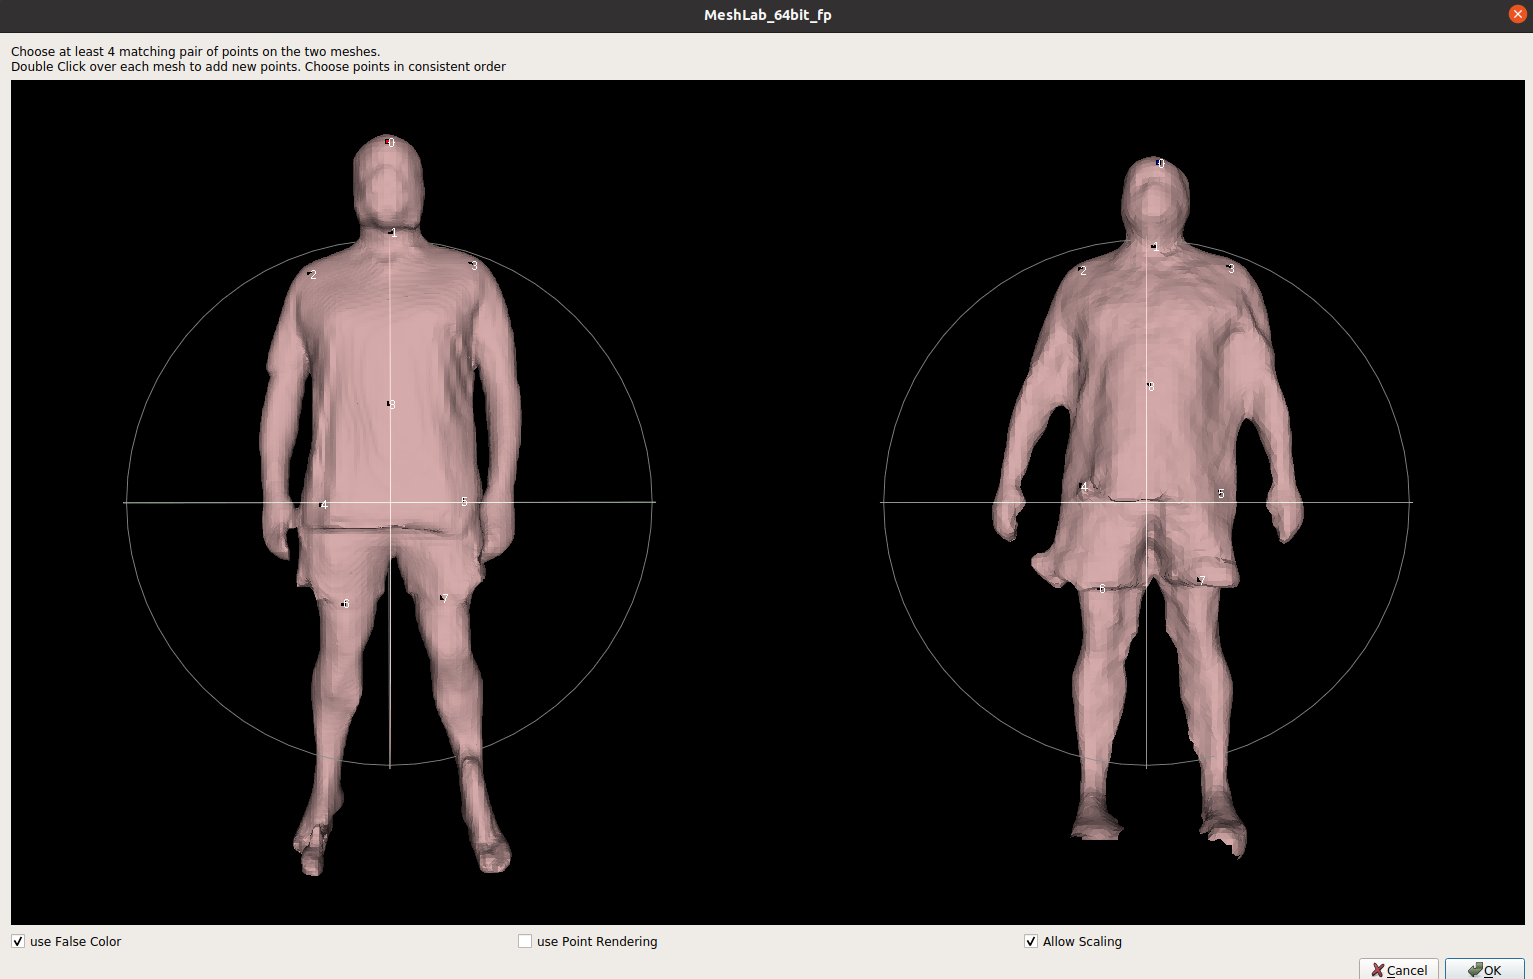
\includegraphics[scale=0.22]{imagenes/alineamiento.png}
	\caption{Proceso alineamiento modelos}
	\label{fig:figura10}
\end{figure}

En la figura \ref{fig:figura10} podemos observar dos modelos, el de la izquierda es el obtenido mediante la red[\cite{pifu}], el de la derecha es el obtenido por Tech4diet[\cite{tech}].

Una vez seleccionados los puntos correctamente y seleccionado $Allow Scaling$ (esta opción se elige porque la red[\cite{pifu}] siempre devuelve un modelo del mismo tamaño, ya que está normalizado), se realiza el alineamiento.

\begin{figure}[H]
	\centering
	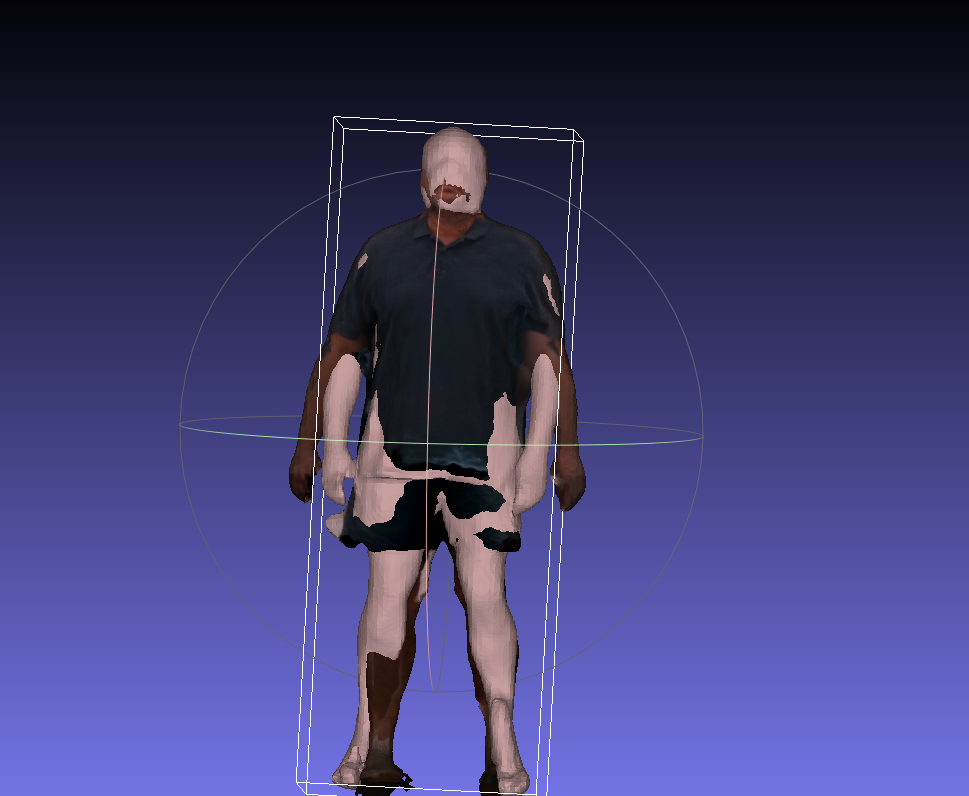
\includegraphics[scale=0.27]{imagenes/alineamiento2.png}
	\caption{Modelos alineados}
	\label{fig:figura11}
\end{figure}

En la figura \ref{fig:figura11} se observa el resultado obtenido después de la alineación.

Con la alineación realizada ya se puede usar la herramienta que nos calcula la distancia de Hausdorff.

\section{Cálculo distancias}

En la comparación de los modelos se han utilizado las distancias de Hausdorff y Chamfer como se ha mencionado con anterioridad, en este punto se va a explicar como se han obtenido las medidas.

\subsection{Distancia Hausdorff}
Como se ha comentado en el punto 4.1, la distancia de Hausdorff de ha calculado mediante la herramienta de MeshLab[\cite{MeshLab}] que te permite calcularla, esta te da un resultado parecido al siguiente: 

\begin{python}
	"Hausdorff Distance computed
	Sampled 58888 pts (rng: 0) on result_camelia0.obj searched closest on Camelia.obj
	min : 0.000000 max 0.339742 mean : 0.020914 RMS : 0.029951
	Values w.r.t. BBox Diag (1.819615)
	min : 0.000000 max 0.186711 mean : 0.011493 RMS : 0.016460"
\end{python}

Donde $min$ dignifica la mínima distancia que hay entre las mallas, $max$ la máxima distancia existente de un punto a otro de las mallas, $mean$ es la media y $RMS$ significa Root Mean Square, que es la raíz cuadrada de la media aritmética de los cuadrado de los valores.

Se ven dos líneas de valores:
\begin{enumerate}
	\item Los datos de la primera línea tienen el valor en la unidad de medida que se esté usando. En este caso hablamos en metros.
	\item Los datos de la segunda línea tienen los valores anteriores pero divididos por la longitud de la diagonal de la bounding box (cuadro delimitador de las mallas), en este caso ese valor es $1.82$. La diagonal que se usa es la de la malla que se usa como referencia por lo tanto en este caso es obtenida por el modelo 3D de Tech4diet[\cite{tech}].
\end{enumerate}

\subsubsection{Quality Mapper}

También se ha usado la herramienta $Quality Mapper$ para observar donde se encuentran las mayores diferencias entre las dos mallas.

Esta herramienta colorea la malla en un gradiente, donde el color rojo significa que es muy distante de la malla y contra más azul oscuro más se acerca una malla a la otra.

Esta herramienta nos ha permitido poder analizar los modelos desde otro punto de vista, pero para poder utilizarlo se ha realizado antes el cálculo de la distancia de Hausdorff con anterioridad.

\begin{figure}[H]
	\centering
	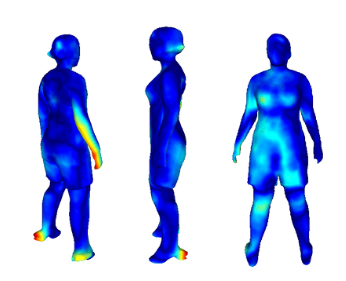
\includegraphics[scale=0.7]{imagenes/qualitymapper.png}
	\caption{Modelos 3D con el gradiente del Quality Mapper.}
	\label{fig:qualitymapper}
\end{figure}

\clearpage
\subsection{Distancia Chamfer}
Para la correcta programación de la distancia Chamfer se ha hecho uso de la siguiente función en Python[\cite{python}]:

\begin{lstlisting}[caption={Código obtención distancia chamfer}, label=cod:3]
\end{lstlisting}
\begin{python}
	def chamfer_distance(x, y, metric='l2'):
	x_nn = NearestNeighbors(n_neighbors=1, leaf_size=1, algorithm='kd_tree', metric=metric).fit(x)
	min_y_to_x = x_nn.kneighbors(y)[0]
	y_nn = NearestNeighbors(n_neighbors=1, leaf_size=1, algorithm='kd_tree', metric=metric).fit(y)
	min_x_to_y = y_nn.kneighbors(x)[0]
	chamfer_dist = np.mean(min_y_to_x) + np.mean(min_x_to_y)
	return chamfer_dist
\end{python}

En el código \ref{cod:3}[\cite{prokudin_2022}] se calcula la distancia media mínima para cada punto que hay de la malla $x$ a la $y$ y viceversa.

\section{Análisis y comparativas de los modelos}

En este punto se analiza y compara los modelos 3D obtenidos mediante el método de PIFu[\cite{pifu}], con tres modelos obtenidos mediante Tech4diet[\cite{tech}]. 

Para ello, se van a utilizar los cálculos explicados con anterioridad, tablas, figuras y gráficas para ayudar a la comprensión.

\begin{figure}[H]
	\centering
	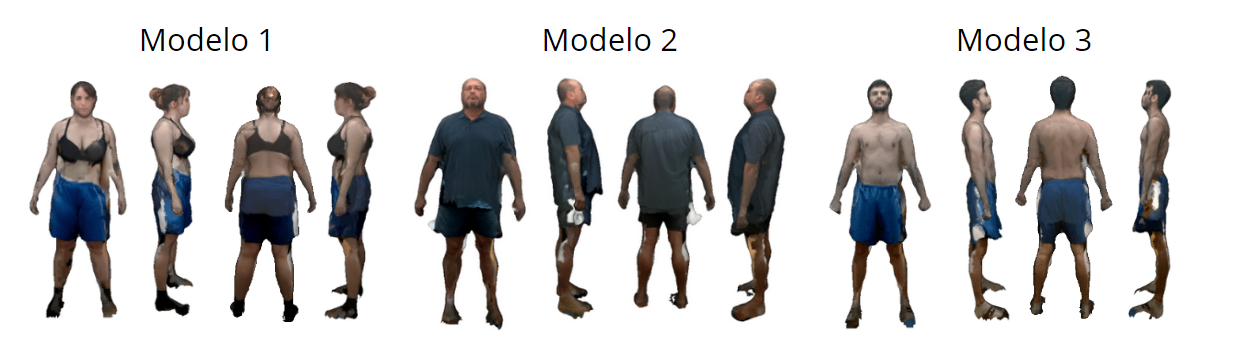
\includegraphics[scale=0.4]{imagenes/t4d.png}
	\caption{Modelos de Tech4diet[\cite{tech}] }
	\label{fig:t4d}
\end{figure}

Primero, el modelo 1, es el cuerpo de una mujer, este modelo ha dado problemas en PIFu[\cite{pifu}] que han ocurrido también en el modelo 2, y es que al estar la red[\cite{pifu}] entrenada con cuerpos normativos, ha sido incapaz de representar correctamente el torso y ha hecho una representación más delgada de lo que es en la realidad.

\begin{figure}[H]
	\centering
	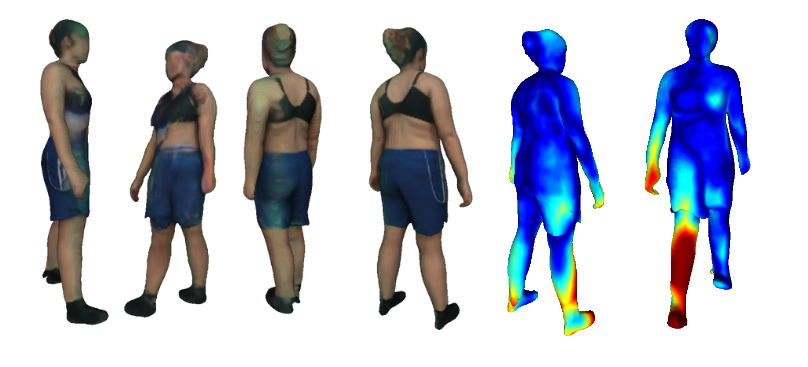
\includegraphics[scale=0.4]{imagenes/cameliadetrasderecha.png}
	\caption{Modelo 1 ángulo diagonal Detrás-Derecha anexo \ref{fig:c4}. Modelo 3D proporcionado por PIFu[\cite{pifu}] y  con Quality Mapper}
	\label{fig:camederechadetras}
\end{figure}

\begin{table}[H]
	\centering
	\caption{Resultados obtenidos con el cálculo de distancias para el modelo 1.}
	\label{table:came}
	\begin{tabular}{l|rrrrrl}
		Modelo 1         & \multicolumn{1}{l}{Figura Anexo} & \multicolumn{1}{l}{min} & \multicolumn{1}{l}{max} & \multicolumn{1}{l}{mean} & \multicolumn{1}{l}{RMS} & Chamfer    \\ 
		\hline
		Frente           & \ref{fig:c1}    & 0,000000                & 0,339742                & 0,020914                 & 0,029951                & 0,2290061  \\
		Detrás Izquierda & \ref{fig:c2}    & 0,000000                & 0,140023                & 0,022127                 & 0,031215                & 0,2221818  \\
		Detrás           & \ref{fig:c3}    & 0,000000                & 0,115258                & 0,018269                 & 0,024125                & 0,2185381  \\
		Detrás Derecha   & \ref{fig:c4}    & 0,000002                & 0,197695                & 0,034686                 & 0,050646                & 0,2191055  \\
		Frente 2         & \ref{fig:c5}    & 0,000003                & 0,163017                & 0,163017                 & 0,029019                & 0,2304320 
	\end{tabular}
\end{table}
\FloatBarrier

\begin{figure}[H]
	\centering
	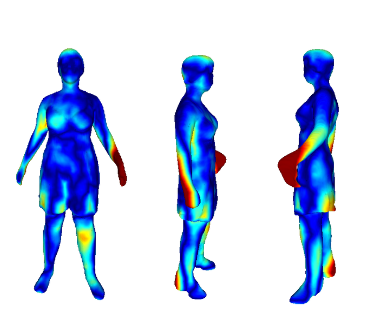
\includegraphics[scale=0.6]{imagenes/cameliafrente.png}
	\caption{Modelo 1 Frente anexo \ref{fig:c1}. Quality Mapper, en tres ángulos diferentes}
	\label{fig:camedelante}
\end{figure}


En lo que se refiere a la distancia de Hausdorff está conformada por $min$, $max$, $mean$ y $RMS$, estos valores tienen como unidad de medida los metros, es decir el en la primera línea de la tabla \ref{table:came} (ángulo de frente) en $max$ el valor de $0,34$ esto significa que el punto más alejado esta a 34 centímetros.
Este valor es alto para un cuerpo humano y se puede observar que el resto los valores son bastante más pequeños y en general más similares entre ellos, como por ejemplo en $mean$. Este valor alto es debido a que un punto o un conjunto de puntos que están más lejos. 

Si se observa el modelo con la figura \ref{fig:camedelante}, se puede identificar la razón de esta distancia. El error está en los brazos, en concreto en la mano, ya que esta deforme y de hecho Quality Mapper nos lo señala también con el color rojo. Aparte de eso existe un problema que ocurre en todos los modelos, y es que la foto no se hizo al mismo tiempo que cuando se hizo la reconstrucción por cabina, y la pose se ha visto modificada, la apertura de las pierna y de los brazos varía en respecto al modelo de Tech4diet[\cite{tech}].

Como se ha comentado al inicio otro de los errores en este modelo es el torso, en general el torso lo ha hecho más delgado, tanto el pecho como la barriga, a diferencia de las piernas que se puede analizar que se han representado bastante bien en comparación a otras representaciones como se puede ver en la figura \ref{fig:camederechadetras}.

Además, en la tabla \ref{table:came} se puede ver que la media de la figura \ref{fig:camederechadetras} es la más alta, por lo tanto la que mejor representada está.

Mencionar que según la distancia de Chamfer el mejor modelo es el que tiene la vista trasera y que para Hausdorff ese es el segundo, por lo tanto este es según las métricas usadas el mejor modelo obtenido.


\begin{figure}[H]
	\centering
	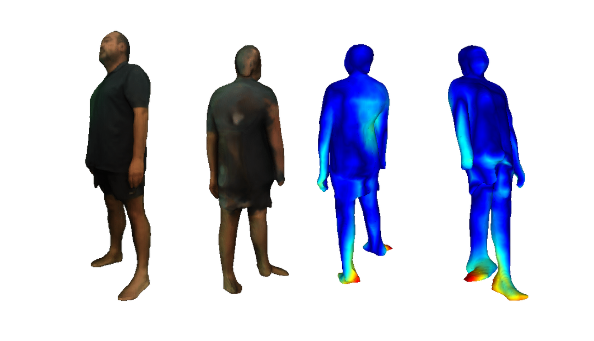
\includegraphics[scale=0.6]{imagenes/andresiz.png}
	\caption{Modelo 2 ángulo diagonal Frente-Izquierda anexo \ref{fig:a2}. Quality Mapper y el modelo obtenido por PIFu[\cite{pifu}] con su textura}
	\label{fig:andresiz}
\end{figure}

\begin{table}[H]
	\centering
	\caption{Resultados obtenidos con el cálculo de distancias para el modelo 2.}
	\label{tablaandres}
	\begin{tabular}{l|rrrrrl}
		Modelo 2         & \multicolumn{1}{l}{Figura Anexo} & \multicolumn{1}{l}{min} & \multicolumn{1}{l}{max} & \multicolumn{1}{l}{mean} & \multicolumn{1}{l}{RMS} & Chamfer    \\ 
		\hline
		Frente           &   \ref{fig:a1}                   & 0,000000                & 0,146557                & 0,02436                  & 0,032245                & 0,2168766  \\
		Frente Izquierda &   \ref{fig:a2}                   & 0,000000                & 0,189554                & 0,029499                 & 0,041392                & 0,2252578  \\
		Frente Derecha   &   \ref{fig:a3}                   & 0,000001                & 0,229704                & 0,032572                 & 0,050265                & 0,2256550  \\
		Detrás           &   \ref{fig:a4}                   & 0,000001                & 0,515040                & 0,039219                 & 0,056044                & 0,1965835 
	\end{tabular}
\end{table}
\FloatBarrier

En este caso vuelve a ocurrir algo similar a lo anterior y es que uno de los modelos que mejor representado está tiene el punto más lejano a 51 centímetros. Esto se debe a que PIFu[\cite{pifu}] ha generado el modelo con un poco de ruido, en la figura \ref{fig:andresdetras} se puede identificar un punto rojo que no forma parte del cuerpo.

Quitado de ese ruido, se puede observar en las cálculos obtenitos que, para Chamfer es el mejor modelo comparado, y con Quality Mapper podemos ver que el resto del modelo es todo celeste y azul oscuro.

En este Modelo 2, vuelve a ocurrir lo comentado en el Modelo 1, y es que se observa la reducción de peso considerable en los modelos, esto es debido a que la red[\cite{pifu}] está entrenada con cuerpos semejantes a los que estamos viendo, en concreto PIFu está entrenada con High-Fidelity Clothed HUman Dataset obtenidos desde [\cite{SiCloPe}, \cite{bodynet}]. 

Las malformidades que también somos capaces de ver en los pies es por la misma razón anterior y es que, trata de hacer zapatillas, tacones o cualquier tipo de zapato, dado que no se ha entrenado con pies descalzos.

\begin{figure}[H]
	\centering
	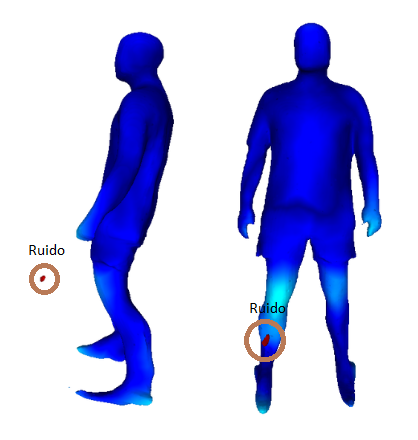
\includegraphics[scale=0.4]{imagenes/andresdetras.png}
	\caption{Modelo 2 Detrás anexo \ref{fig:a4}. Quality Mapper señalando el error}
	\label{fig:andresdetras}
\end{figure}

El último modelo en general ha obtenido mejores resultados ya que se trata de un hombre con cuerpo normativo, por lo tanto la red[\cite{pifu}] sabe comportarse mejor a este tipo de cuerpo ya que está entrenada para ello.

\begin{figure}[H]
	\centering
	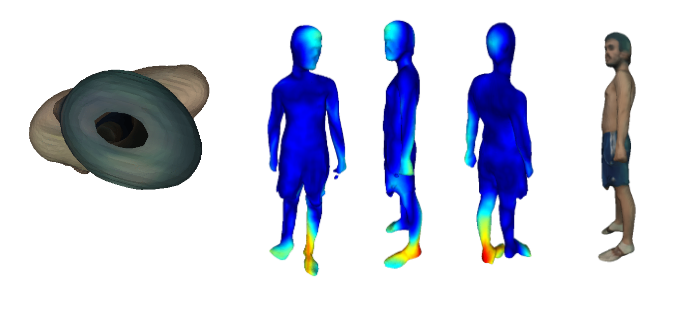
\includegraphics[scale=0.5]{imagenes/nahuelado.png}
	\caption{Modelo 3 Frente-Izquierda anexo \ref{fig:n2}. La primera imagen es un error existente en la cabeza. Las tres siguientes diferentes ángulos con Quality Mapper y la ultima el modelo obtenido con PIFu[\cite{pifu}]}
	\label{fig:nahuelado}
\end{figure}

\begin{table}[H]
	
	\begin{tabular}{l|rrrrrl}
		Modelo 3         & \multicolumn{1}{l}{Figura Anexo} & \multicolumn{1}{l}{min} & \multicolumn{1}{l}{max} & \multicolumn{1}{l}{mean} & \multicolumn{1}{l}{RMS} & Chamfer    \\ 
		\hline
		Frente           &   \ref{fig:n1}                   & 0,000001                & 0,408629                & 0,036266                 & 0,059013                & 0,1848258  \\
		Frente Izquierda &   \ref{fig:n2}                   & 0,000000                & 0,209037                & 0,029888                 & 0,046514                & 0,2001989  \\
		Detrás		     &   \ref{fig:n3}                   & 0,000001                & 0,124862                & 0,029777                 & 0,037247                & 0,1641800  
	\end{tabular}
	\caption{Resultados obtenidos con el cálculo de distancias para el modelo 3.}
	\label{tablanahuel}	
\end{table}
\FloatBarrier

Como se puede observar aunque los valores son más pequeños, aún existen errores, por ejemplo en la representación del ángulo Frente-Izquierda \ref{fig:nahuelado} nos encontramos varios, en este caso la cabeza es muy grande, el cuerpo esta ladeado, las piernas hay una más corta que la otra, los pies los representa con errores también y hay un hueco en la cabeza. 

Es el único modelo de PIFu[\cite{pifu}] que se ha encontrado con un error tan grande como la falta de superficie en alguna parte. Es por ello que tanto para Chamfer, como para Hausdorff los valores no hayan sido más bajos, ya que falta información.

Y por último en el modelo 3, mencionar que se encuentra el mejor resultado de Chamfer que es 0,16, en esta figura \ref{fig:nahuel} no se le ven muchos errores de primer vistazo, por lo que se le ha tenido que subir la capacidad de reconocer diferencias en Quality Mapper a diferencia del resto, en este modelo se puede observar que sigue teniendo problemas reconociendo los pies, y trata de hacer zapatillas, las manos a diferencia del resto están muy bien.

\begin{figure}[H]
	\centering
	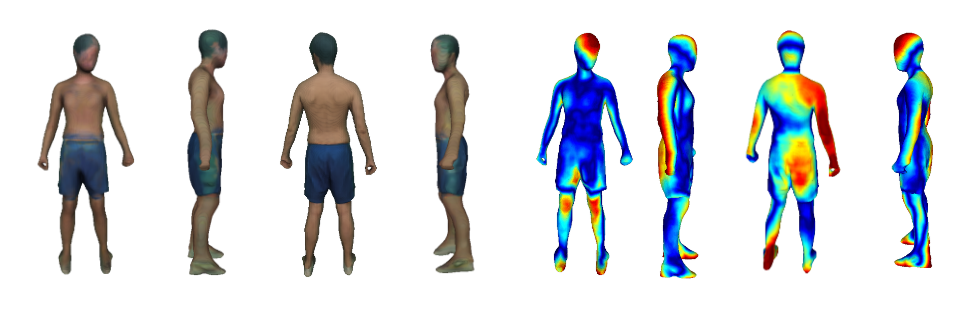
\includegraphics[scale=0.5]{imagenes/nahuel.png}
	\caption{Modelo 3 Detrás anexo \ref{fig:n3}. Modelo obtenido por PIFu[\cite{pifu}] y Quality Mapper.}
	\label{fig:nahuel}
\end{figure}

\begin{figure}[H]
	\centering
	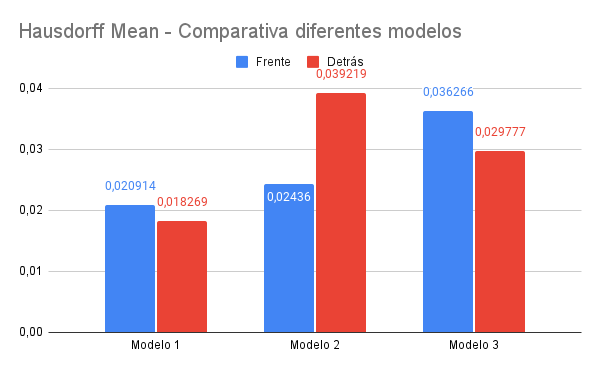
\includegraphics[scale=0.5]{imagenes/Hausdorff-difmods.png}
	\caption{Gráfica comparativa de los 3 modelos, con el cálculo de la distancia de Hausdorff. Con los ángulos de frente y detrás}
	\label{fig:haus}
\end{figure}
\begin{figure}[H]
	\centering
	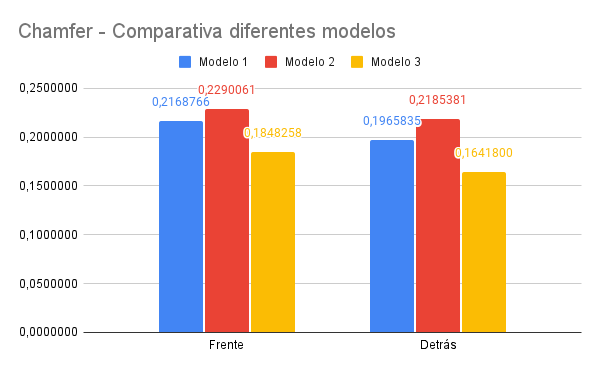
\includegraphics[scale=0.5]{imagenes/Chamfer-difmods.png}
	\caption{Gráfica comparativa de los 3 modelos, con el cálculo de la distancia de Chamfer. Con los ángulos de frente y detrás}
	\label{fig:cham}
\end{figure}

En las gráficas \ref{fig:haus} y \ref{fig:cham} se comprueba lo anteriormente analizado, y es que el modelo 3 ha obtenido mejores resultados que el resto.

Una de las conclusiones que obtenemos después de este análisis es que, los modelos 3D generados a partir de una imagen 2D con vista en diagonal, obtiene malos resultados. De estos modelos, solo se ve bien desde el ángulo de la foto, el resto de ángulos PIFu[\cite{pifu}] no los comprende, y cuando lo recompone, entiende que lo que ocurre es que hay una pierna más corta que otra o un brazo mas largo que otro, o la espalda muy girada.

Destacar que la infirencia sobre la textura en los modelos ha sido muy buena, incluso en las imágenes de espalda como se ve en la figura \ref{fig:nahuel}, es capaz de reconocer que esta de espaldas e inferir en la cara un color de piel obtenido del cuerpo.

Para finalizar se puede observar que en ambas distancias se obtienen buenos resultados, pero no para el ámbito en el que nos encontramos que es el dietético-nutricional.
Este ámbito requiere de una precisión que no se ha obtenido, ya que realmente todos los modelos se han visto de una manera u otra modificados.